\chapter{General trends}
\label{ch:general}

\section{Onboard temperature ($T_\mathrm{cal}$)}
\label{sec:Tcal}

\begin{figure}[ht]
    \centering
    \begin{subfigure}[b]{0.9545\textwidth}
        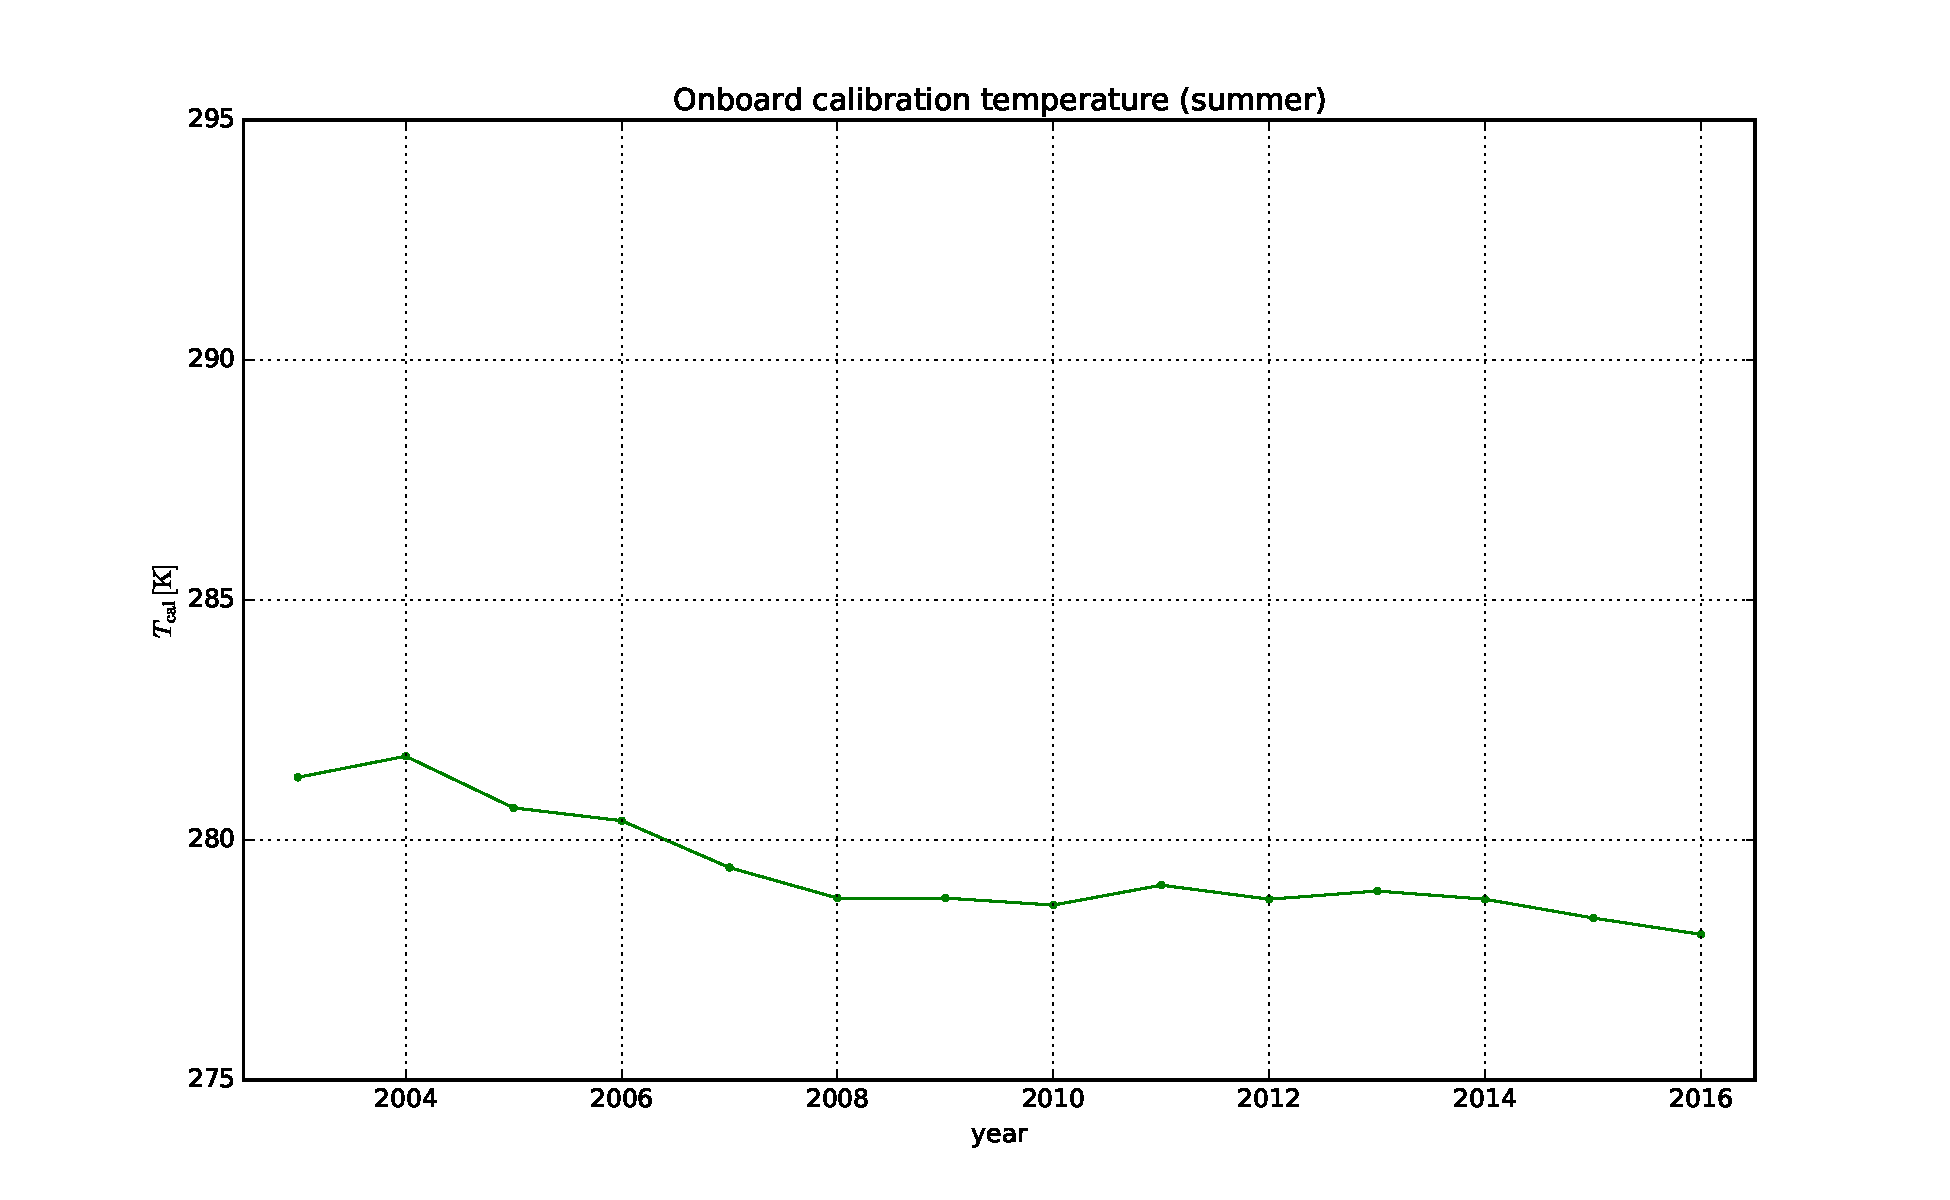
\includegraphics[width=\textwidth]{misc/tcal_summer}
        \caption{summer}\label{fig:tcal:summer}
    \end{subfigure}
    \begin{subfigure}[b]{0.9545\textwidth}
        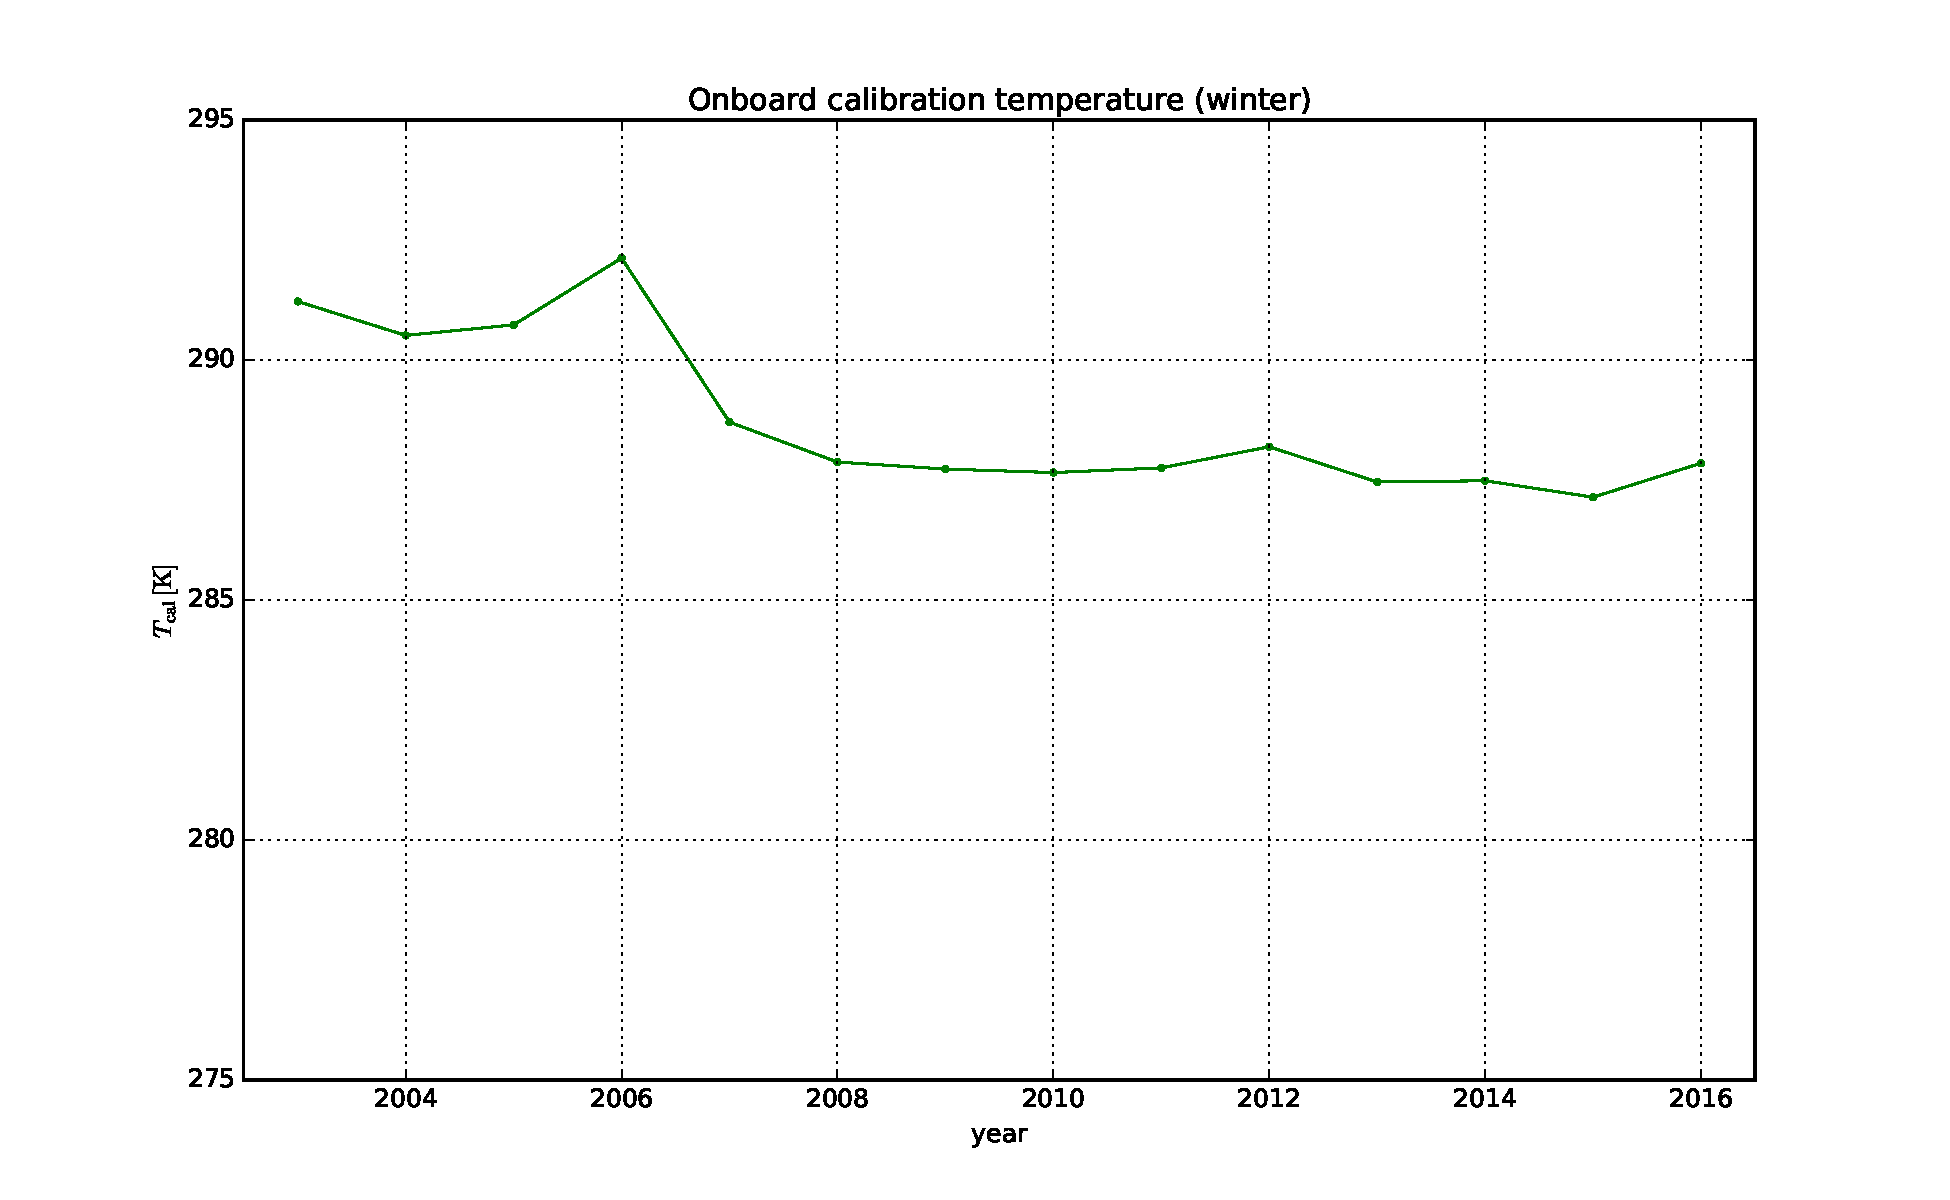
\includegraphics[width=\textwidth]{misc/tcal_winter}
        \caption{winter}\label{fig:tcal:winter}
    \end{subfigure}
    \caption{Median calibration temperatures ($T_\mathrm{cal}$) for
        summer~(cold) and winter~(warm) from 2003 to 2016. $T_\mathrm{cal}$ is
        useful as a proxy for the overall onboard temperature on the Odin
        satellite.}\label{fig:tcal}
\end{figure}

\noindent
Fig.~\ref{fig:tcal} shows how the median calibration temperature
($T_\mathrm{cal}$) has varied over time from 2003 to 2016.  $T_\mathrm{cal}$ is
useful as a proxy for the overall onboard temperature on the Odin satellite.
Odin is at its coldest around the arctic midsummer, and at its warmest during
the the arctic midwinter.  As can be seen in the figure the temperature
difference is approximately $9\,\mathrm{K}$.  With the exception of the
winter 2006, the temperature has been on a decline since the start of the
mission, but most of the drop occured before 2008, which coincides with the
period when the astronomy mission was active.  After 2008 there is only a hint
of a downward trend, which may be attributable to confirmation bias.


\section{Receiver temperature ($T_\mathrm{rec}$)}
\label{sec:Trec}
Fig.~\ref{fig:trec} shows how the median receiver temperature
($T_\mathrm{rec}$) has varied over time from 2003 to 2016 for all the studied
frequency modes.  The trends are not the same for all modes, owing to them
having different frontends (see~\ref{table:config4}), but for several modes,
in particular for FM~01 and~02, a difference in the trend can be seen comparing
the period before and after $\sim$2009, which corresponds to the periods where
we see changes in the behaviour of the spectra.  This might indicate the same
root cause for the different phenomena.

\begin{figure}[ht]
    \centering
    \begin{subfigure}[b]{0.9545\textwidth}
        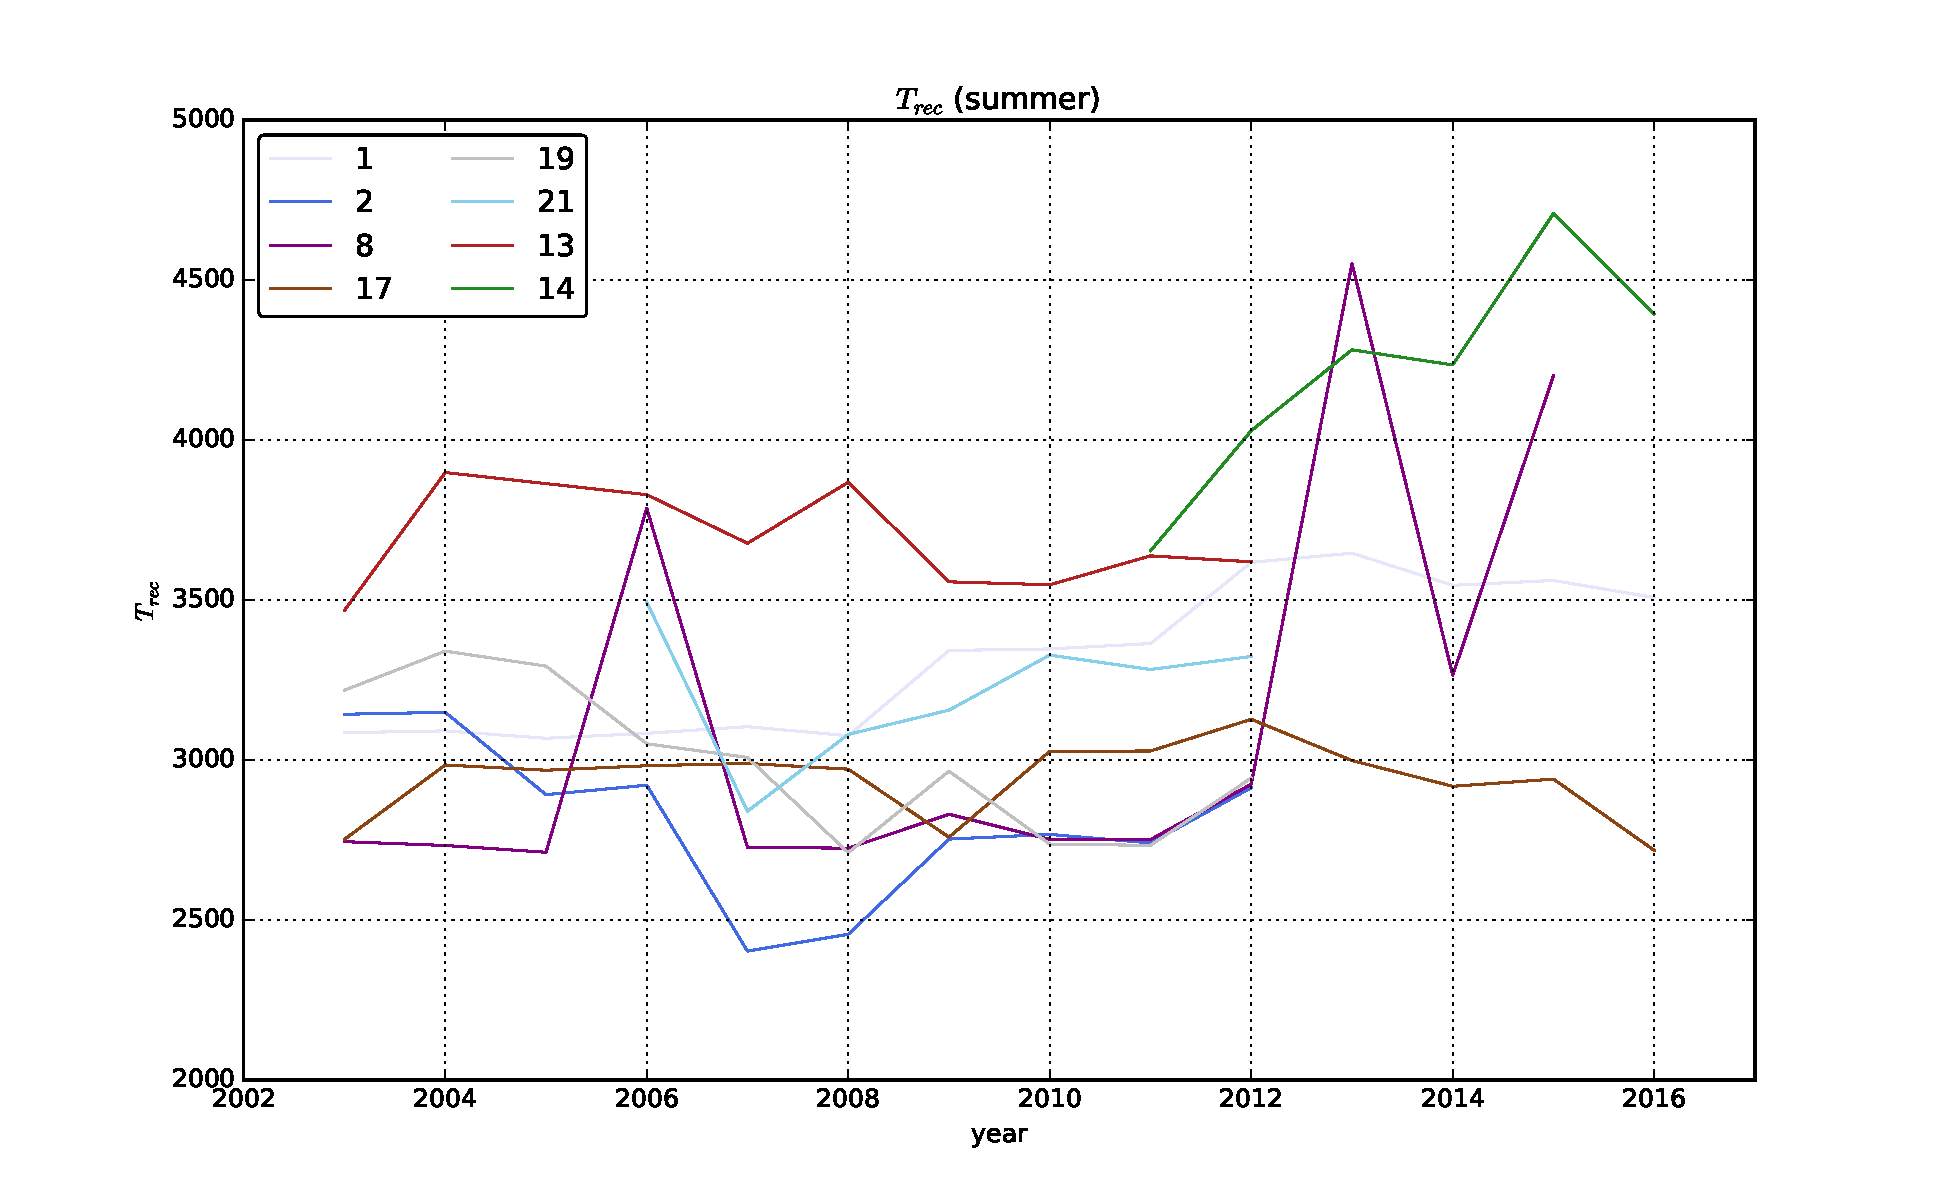
\includegraphics[width=\textwidth]{misc/trec_summer_all}
        \caption{summer}\label{fig:01:trec:summer}
    \end{subfigure}
    \begin{subfigure}[b]{0.9545\textwidth}
        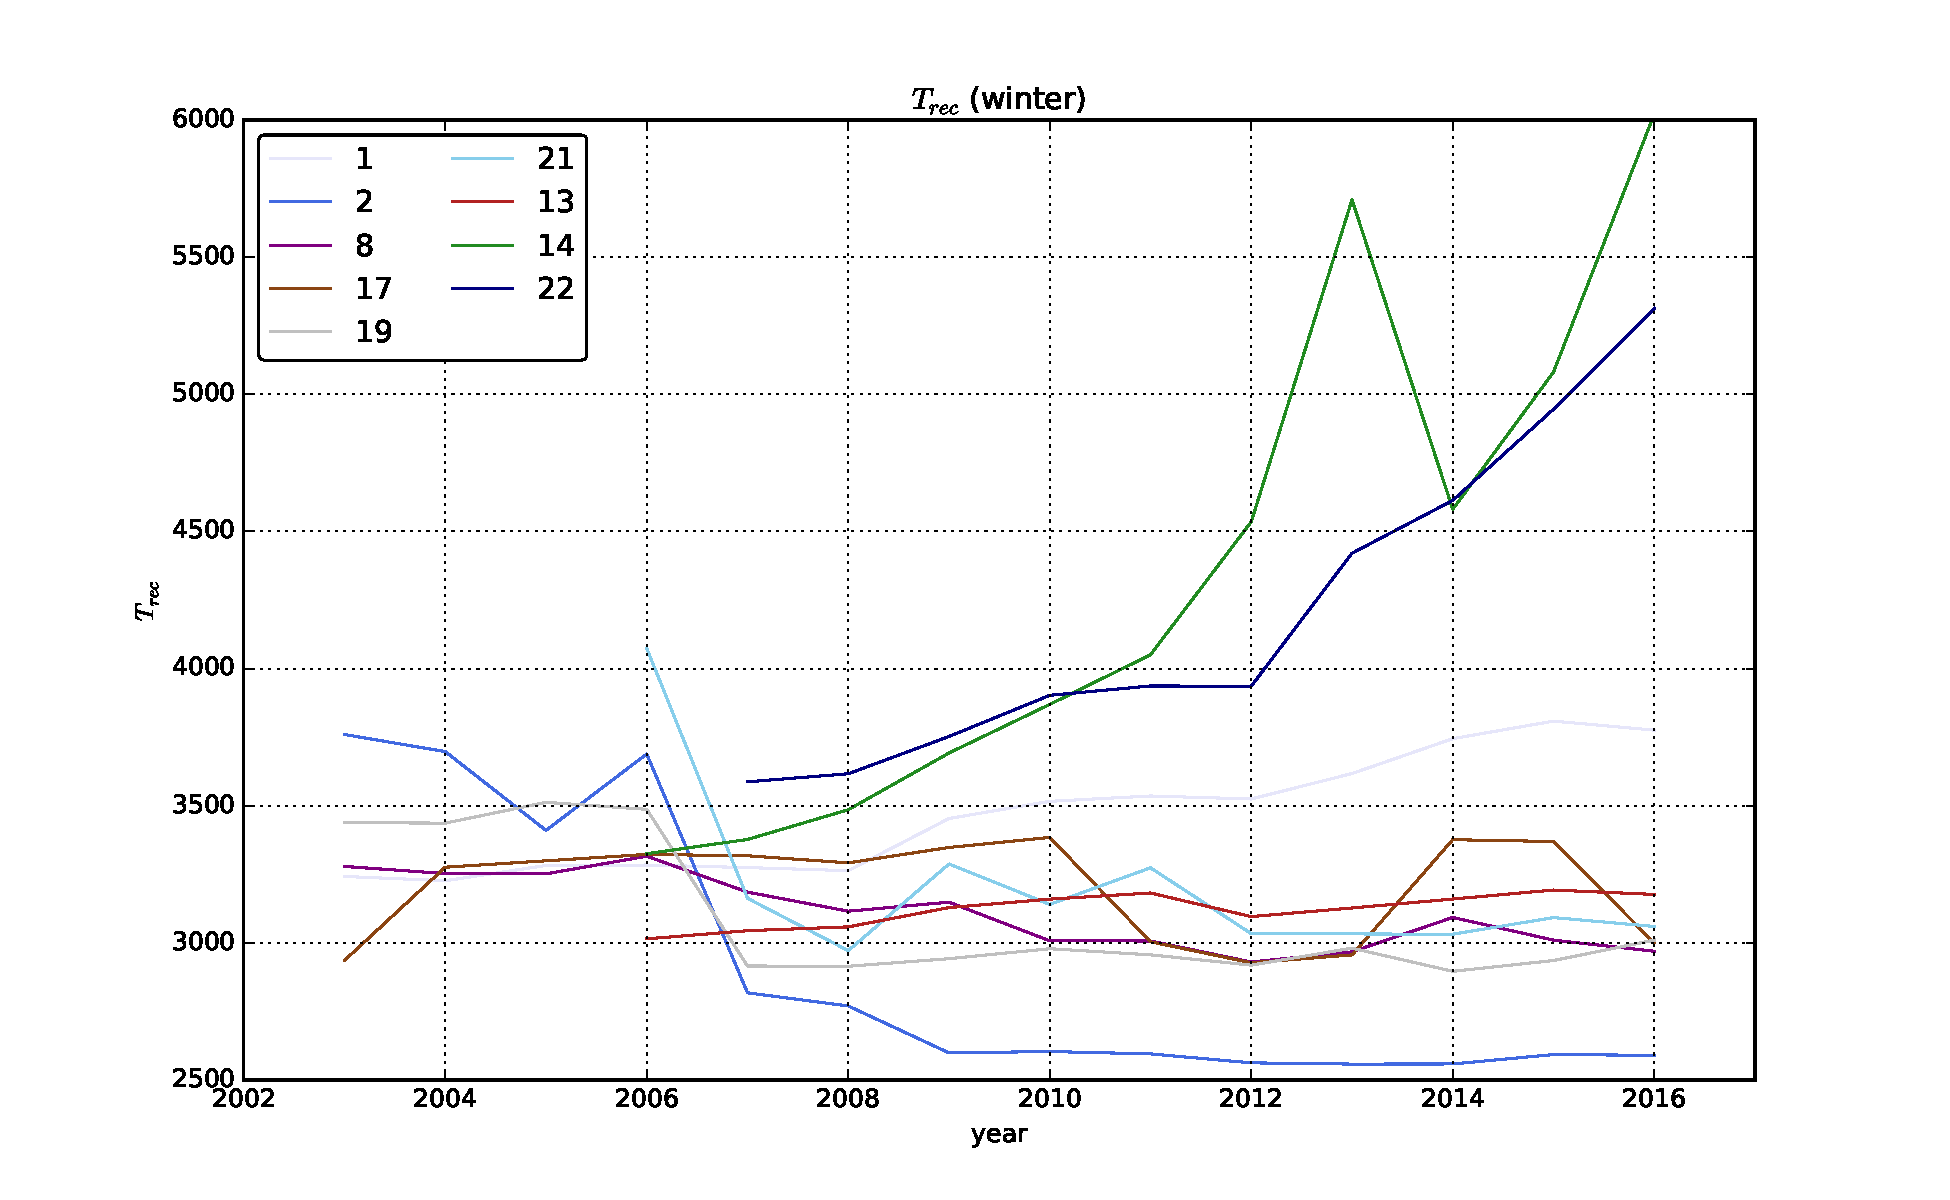
\includegraphics[width=\textwidth]{misc/trec_winter_all}
        \caption{winter}\label{fig:01:trec:winter}
    \end{subfigure}
    \caption{Median receiver temperatures ($T_\mathrm{rec}$) for
        summer~(cold) and winter~(warm) from 2003 to 2016.
        }\label{fig:trec}
\end{figure}
